\documentclass[a4paper,12pt]{article}
\usepackage[utf8]{inputenc}
\usepackage{amsmath, amssymb}
\usepackage{graphicx}
\usepackage{float}
\usepackage{tikz}
\usepackage{listings}
\usepackage{xcolor}
\usepackage{caption}
\usepackage{geometry}
\geometry{margin=1in}

\title{Big Assignment: Object-Oriented Programming\\\large Design of Project}
\author{Yusupov Boburjon\\Neptun Code: YTAJDI}
\date{April 18, 2024}
\captionsetup[figure]{labelformat=empty} % Remove figure label

\begin{document}

\maketitle

\newpage

\section*{1. Project description: Wildlife Simulation}

Wildlife conservation is the most critical issue in a major game reserve.  
Trained rangers venture out daily to spot wildlife, administer medicine to diseased animals, and protect the habitat from desecrating poachers. The reserve is a well-organized company where rangers, animals, habitats, and support vehicles coexist in symbiosis for fostering nature’s fragile balance.

All animals have a species, health, and a stress level. Animals become stressed or injured due to natural events or poachers. The rangers can calm them down and treat them.

Rangers are diligent workers who protect the reserve’s environment. Every ranger has a name, experience, and efficiency. They can assist an animal by improving its status or reducing stress. They can also detect animals that need help among all the animals and help them. If they are in the same habitat as a poacher, they find and fight the poacher. The winner is determined based on the strength of both the ranger and the poacher. The strength is initialized randomly.

Poachers are intruders who hunt down animals. Each poacher targets a specific species. Different poachers are dangerous to a different degree. Poachers disturb wildlife and cause them stress as they evade their hunters. They can also hurt the animals if they catch them.

Each habitat has a name, a capacity, and the animals living in it. Animals can enter and leave habitats. If there is an incursion by a poacher, it stresses all animals in the habitat.

The rangers travel in Jeep vehicles. The vehicle has an ID, fuel level, and a capacity. Vehicles can be refueled and deployed to specific habitats.

The simulation is run day-by-day. Each day, animals wander between habitats, rangers are sent to habitats to patrol them, and poachers go to habitats to hunt animals. The simulation reports at the end of the day the state of the reserve and the happenings on that day — for example, what animals were saved.

Play it out, roll out your rangers, and save the wildlife!

\bigskip

\textbf{Input file examples}

\textbf{\texttt{animals.txt}}
\begin{itemize}
    \item Format
    \newline \text{Species Health StressLevel}
    \item Example
    \begin{verbatim}
        Elephant 60 30
        Giraffe 70 20
        Zebra 80 25
    \end{verbatim}
\end{itemize}

\textbf{\texttt{rangers.txt}}
\begin{itemize}
    \item Format
    \newline \text{Name Experience Efficiency}
    \item Example
    \begin{verbatim}
        Balazs 5 7
        Sofiia 6 6
    \end{verbatim}
\end{itemize}

\textbf{\texttt{vehicles.txt}}
\begin{itemize}
    \item Format
    \newline \text{ID FuelLevel Capacity}
    \item Example
    \begin{verbatim}
        V1 100 2
        V2 100 3
    \end{verbatim}
\end{itemize}

\textbf{\texttt{habitats.txt}}
\begin{itemize}
    \item Format
    \newline \text{Name Capacity}
    \item Example
    \begin{verbatim}
        Savannah 3
    \end{verbatim}
\end{itemize}

\newpage
\section*{\centering 2. Use Case Diagram}

\begin{figure}[H]
    \centering
    \fbox{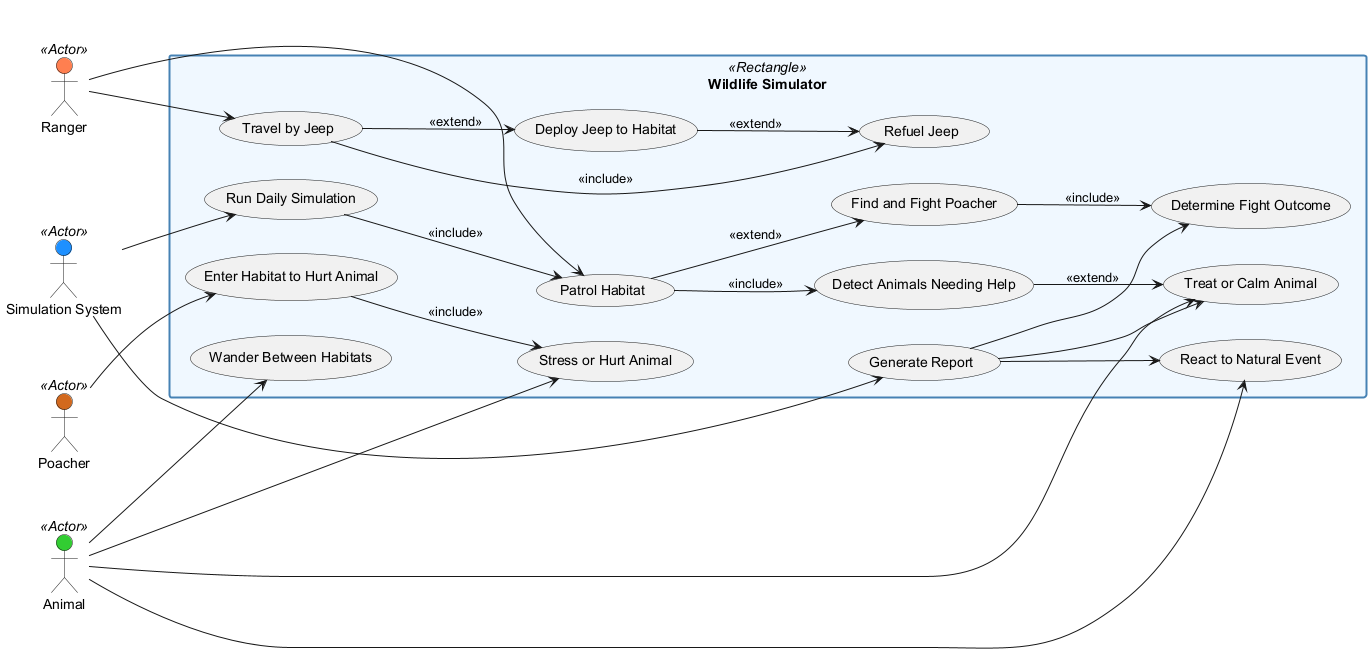
\includegraphics[width=0.9\textwidth]{use-case.png}}
    \caption{Use Case Diagram}
    \label{fig:use-case}
\end{figure}

\noindent Use case diagram shows the interactions between the actors (Ranger, Poacher, Vehicle) and the system (Wildlife Simulation). The actors perform various actions such as patrolling, treating animals, hunting, and moving between habitats. The system manages the habitats, animals, and vehicles.

\bigskip

\begin{flushleft}
\textbf{\large Ranger}:
\begin{itemize}
    \item Patrols the habitat to check for poachers and animals in need of help.
    \item Treats animals to improve their health and reduce stress.
    \item Fights poachers if they confront them in the same habitat.
    \item Moves between habitats to assist animals and patrol areas.
    \item Uses Jeep to travel between habitats.
    \item Refuels and deploys the Jeep to specific habitats.
\end{itemize}

\bigskip

\textbf{\large Poacher}:
\begin{itemize}
    \item Incurses in the habitat to hunt animals.
    \item Hurts animals if they catch them and lowers their health level.
    \item Stresses animals in the habitat and increases their stress level.
    \item Moves between habitats to hunt animals.
    \item Fights rangers if they confront them in the same habitat.
\end{itemize}
\end{flushleft}
\end{document}
